% Adaptive Cyber-Physical Anomaly Detection — NSL-KDD + MAE + One-Class SVM
% Build: see README.md in this directory (pdflatex + bibtex).
\documentclass[11pt,a4paper]{article}

\usepackage[T1]{fontenc}
\usepackage[utf8]{inputenc}
\usepackage{lmodern}
\usepackage{microtype}
\usepackage{amsmath,amssymb,bm}
\usepackage{booktabs}
\usepackage{graphicx}
\usepackage{tikz}
\usetikzlibrary{arrows.meta,positioning,fit,calc}
\usepackage{hyperref}
\hypersetup{colorlinks=true,linkcolor=blue!55!black,citecolor=blue!55!black,urlcolor=blue!55!black}
\usepackage[round,authoryear]{natbib}
\usepackage{cleveref}
\usepackage{geometry}
\geometry{margin=1in}

\title{\textbf{Learning a Margin of Normalcy for Zero-Day Network Intrusion Detection:\\
Masked Autoencoders and One-Class SVMs on NSL-KDD Flow Features}}
\author{%
  Kartik Yadav\\
  Agrapujya Lashkari\\[0.75em]
  \textit{Rishihood University}%
}
\date{\today}

\begin{document}
\maketitle

\begin{abstract}
Signature-based intrusion detection systems fail silently against \emph{zero-day} attacks for which no templates exist. We frame enterprise and industrial monitoring as \emph{semi-supervised anomaly detection}: models observe only benign connection traffic during training and score deviations at deployment. On the NSL-KDD benchmark, we combine (i) skew-driven logarithmic transforms with scalable one-hot encoding, (ii) a tabular masked autoencoder trained with a BERT-style masked reconstruction objective, (iii) RBF one-class SVMs in both raw feature space and learned latent space, and (iv) a calibrated hybrid score. Using the standard NSL train/test protocol with a stratified validation split for threshold selection, we obtain test ROC-AUC of $0.942$ for reconstruction-based detection and $0.920$ for one-class SVM on raw features; a na\"ive linear fusion of reconstruction error and latent SVM margin \emph{degrades} ranking quality (ROC-AUC $0.781$), which we analyse as a failure mode of score aggregation under heterogeneous scales. These results support reconstruction and kernel methods as strong baselines while motivating more principled fusion for hybrid designs.
\end{abstract}

\noindent\textbf{Keywords:} anomaly detection, NSL-KDD, masked autoencoder, one-class SVM, semi-supervised learning, cyber-physical security.

% ------------------------------------------------------------------
\section{Introduction}
\label{sec:intro}

The earliest articulation of \emph{intrusion detection} as an auditing problem dates to threat-monitoring surveys \citep{anderson1980threats}. Operational systems soon split into \emph{misuse} (signature) and \emph{anomaly} branches \citep{lippmann2000progress}. Signatures excel when attack artefacts are stable, but industrial IoT and enterprise backbones now face adversaries who weaponise unknown vulnerabilities---where no string match exists, the defender must infer \emph{normality} and treat strong departures as incidents \citep{chandola2009anomaly}.

This work defends a concrete response to that gap. We do \emph{not} claim to classify attack families; we ask whether a pipeline trained \textbf{only on benign} TCP/IP flow statistics can separate normal connections from attacks on a public benchmark. Our narrative follows three ideas from the literature: (1)~\emph{support estimation} via one-class kernels \citep{scholkopf2001estimating,tax2004support}, (2)~\emph{denoising} representations that compress routine traffic \citep{vincent2008extracting}, and (3)~\emph{masked prediction} as a self-supervised signal \citep{devlin2019bert}, adapted here to \emph{tabular} flow vectors rather than token sequences.

We use NSL-KDD \citep{tavallaee2009detailed}, a curated revision of the KDD Cup~'99 corpus that reduces duplicate flows and sharpens evaluation. We are explicit about limitations stressed by \citet{mahoney2002learning}: traffic is non-stationary, and the NSL train/test split is a \emph{research protocol}, not a guarantee of i.i.d.\ deployment data. Within that honest scope, we report reproducible metrics and a \emph{failure analysis} of our hybrid stage.

\paragraph{Contributions.}
\begin{itemize}\itemsep=0.15em
  \item A semi-supervised pipeline: preprocessor fit on benign rows only; masked autoencoder; one-class SVMs on $\bm{x}$ and on latent $\bm{z}$; hybrid score with validation-tuned convex weight.
  \item Empirical ablation on NSL-KDD (Models~A/B/C) with auxiliary Mahalanobis, GMM, and max-$|z|$ baselines.
  \item Analysis of hybrid under-performance: fusion of non-comparable scores harms ROC ranking despite high precision.
\end{itemize}

% ------------------------------------------------------------------
\section{Dataset and exploratory analysis}
\label{sec:data}

\paragraph{NSL-KDD.} Each record aggregates one logical connection: duration, protocol/service/flag symbols, byte counts, rate statistics, and host-level counters \citep{tavallaee2009detailed}. We use \texttt{KDDTrain+\_20Percent} for development-speed training and the full \texttt{KDDTest+} for reporting, matching common coursework practice. Labels are collapsed to binary: \emph{normal} vs.\ \emph{attack}.

\paragraph{Patterns that drive preprocessing.} Exploratory analysis (correlation heatmaps and kernel density estimates by label) reveals heavy-tailed count-like fields (e.g., \texttt{num\_root}, \texttt{num\_compromised}) with extreme skew. Heavy tails inflate variance under Euclidean metrics and destabilise covariance estimates in high dimension after one-hot expansion. We therefore apply $\log(1+x)$ to the top-$k$ skewed numeric columns \emph{selected on the training split only}, then median imputation and standardisation for numeric columns and dummy encoding for symbolic fields. The \texttt{ColumnTransformer} is \textbf{fit exclusively on benign training rows} so attack statistics do not leak into location/scale estimates.

\paragraph{Caveats.} Attack classes are heterogeneous; treating them as a single ``out'' distribution simplifies evaluation but obscures per-family behaviour. Temporal correlation across flows is ignored---a known weakness of row-wise benchmarks \citep{mahoney2002learning}.

\begin{figure}[t]
  \centering
  \IfFileExists{../reports/figures/phase1_nsl_corr.png}{%
    \includegraphics[width=0.85\linewidth]{../reports/figures/phase1_nsl_corr.png}}{%
    \fbox{\parbox[c][0.35\textheight][c]{0.85\linewidth}{\centering
      \vspace{2em}\textit{Run the project notebook to generate \texttt{reports/figures/phase1\_nsl\_corr.png}.}\vspace{2em}}}}%
  \caption{Pearson correlation among numeric NSL-KDD features (training sample). Block structure motivates regularised distance metrics (Section~\ref{sec:methods}).}
  \label{fig:corr}
\end{figure}

\begin{figure}[t]
  \centering
  \IfFileExists{../reports/figures/phase1_nsl_kde_duration.png}{%
    \begin{minipage}[t]{0.48\linewidth}
      \centering
      \includegraphics[width=\linewidth]{../reports/figures/phase1_nsl_kde_duration.png}\\[-0.2em]
      {\small Duration by label}
    \end{minipage}\hfill
    \begin{minipage}[t]{0.48\linewidth}
      \centering
      \IfFileExists{../reports/figures/phase1_nsl_kde_src_bytes.png}{%
        \includegraphics[width=\linewidth]{../reports/figures/phase1_nsl_kde_src_bytes.png}\\[-0.2em]
        {\small Source bytes by label}}{%
        \fbox{\parbox[c][0.22\textheight][c]{\linewidth}{\centering\textit{Generate KDE plots via notebook.}}}}
    \end{minipage}
  }{%
    \fbox{\parbox[c][0.2\textheight][c]{0.9\linewidth}{\centering\textit{Run the project notebook to generate KDE figures under \texttt{reports/figures/}.}}}}%
  \caption{Label-conditional KDEs for selected heavy-tailed fields (after optional $\log(1{+}x)$ in pipeline). Separation visible on duration and byte volume motivates skew-aware transforms.}
  \label{fig:kde}
\end{figure}

% ------------------------------------------------------------------
\section{Methods}
\label{sec:methods}

\subsection{Baselines and advanced classical detectors}
Let $\bm{x}_i \in \mathbb{R}^d$ denote the preprocessed feature vector. On benign training indices $\mathcal{N}$, we compute column means $\bm{\mu}$ and standard deviations $\bm{\sigma}$ and score $\max_j |(x_{ij}-\mu_j)/\sigma_j|$ (max-$|z|$). For Mahalanobis distance, we employ Ledoit--Wolf shrinkage of the covariance to stabilise $\bm{\Sigma}^{-1}$ when $d$ is large \citep{ledoit2004well,chandola2009anomaly}. For a diagonal-covariance Gaussian mixture with $K$ components, we maximise the expected complete-data log-likelihood via EM \citep{chandola2009anomaly}; $K$ is chosen by BIC on benign data. Anomaly scores are negative log-likelihood. Finally, the $\nu$-SVM one-class formulation \citep{scholkopf2001estimating} with RBF kernel defines a smooth decision boundary in a reproducing kernel Hilbert space; we use $\nu=0.08$ and $\gamma=\texttt{scale}$ as a first-pass configuration.

\subsection{Masked autoencoder (Model~B)}
We use a two-hidden-layer MLP encoder--decoder with batch normalisation, dropout, and Xavier initialisation. During training, a random mask $\bm{m}_i \in \{0,1\}^d$ with fixed masking probability masks coordinates of $\bm{x}_i$; the network predicts the original vector and minimises mean squared error \emph{only on masked entries}---a direct analogue of masked language modelling \citep{devlin2019bert,vincent2008extracting}. Optimisation uses AdamW with weight decay; early stopping monitors masked validation loss on benign validation traffic. At test time, reconstruction error is the mean squared error over \emph{all} coordinates for a full forward pass, yielding a scalar anomaly score per flow.

\subsection{Latent one-class SVM and hybrid (Model~C)}
Encoder outputs $\bm{z}_i \in \mathbb{R}^{d_z}$ are frozen. A second RBF one-class SVM is fit on benign $\bm{z}$ after per-feature standardisation. Reconstruction scores $r_i$ and SVM margin scores $s_i$ are min--max normalised using statistics from \emph{benign validation} rows only, then combined as $h_i = w r_i + (1-w)s_i$ with $w$ selected on a coarse grid to maximise validation F1 at an F1-optimal threshold.

\subsection{Training protocol and metrics}
We hold out a stratified $15\%$ validation slice of the training file for threshold tuning. For each model, we choose the threshold maximising F1 on validation, then report ROC-AUC, PR-AUC (average precision), precision, recall, and F1 on \texttt{KDDTest+}. ROC-AUC summarises ranking quality independent of the chosen threshold.

% ------------------------------------------------------------------
\begin{figure}[t]
  \centering
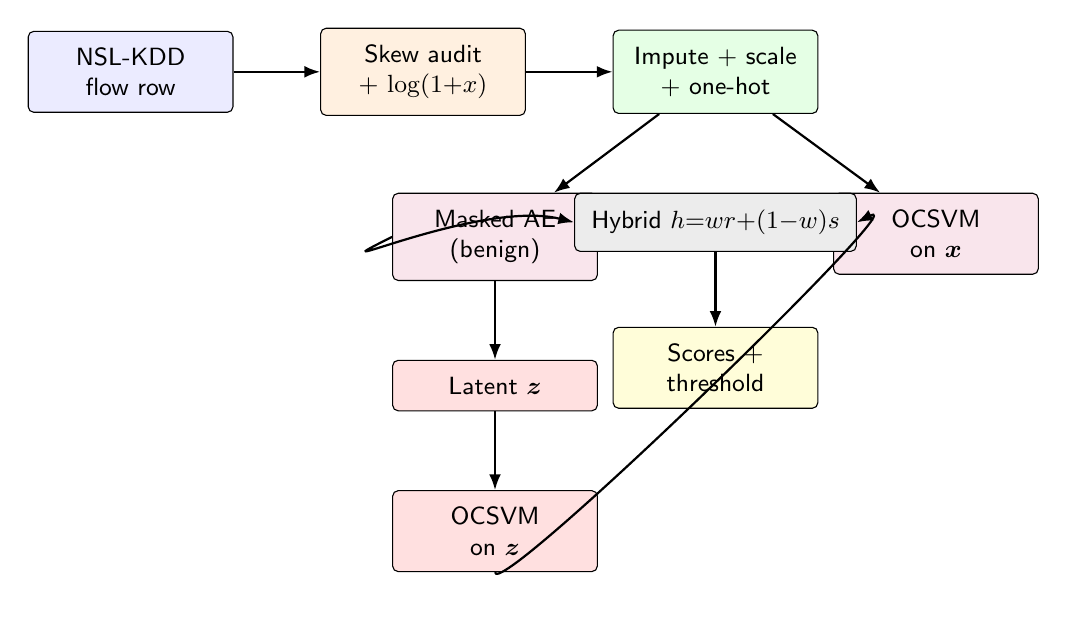
\begin{tikzpicture}[
  font=\small\sffamily,
  box/.style={draw,rounded corners=2pt,align=center,inner sep=6pt,minimum width=2.6cm},
  arrow/.style={-{Latex[length=2mm]},thick}
]
\node[box,fill=blue!8] (nsl) {NSL-KDD\\flow row};
\node[box,fill=orange!12,right=1.1cm of nsl] (fe) {Skew audit\\+ $\log(1{+}x)$};
\node[box,fill=green!10,right=1.1cm of fe] (ct) {Impute + scale\\+ one-hot};
\node[box,fill=purple!10,below=1.0cm of ct,xshift=-2.8cm] (mae) {Masked AE\\(benign)};
\node[box,fill=purple!10,below=1.0cm of ct,xshift=2.8cm] (svmx) {OCSVM\\on $\bm{x}$};
\node[box,fill=red!12,below=1.0cm of mae] (z) {Latent $\bm{z}$};
\node[box,fill=red!12,below=1.0cm of z] (svmz) {OCSVM\\on $\bm{z}$};
\node[box,fill=gray!15,below=1.0cm of ct] (hy) {Hybrid $h{=}wr{+}(1{-}w)s$};
\node[box,fill=yellow!15,below=0.95cm of hy] (out) {Scores +\\threshold};
\draw[arrow] (nsl) -- (fe);
\draw[arrow] (fe) -- (ct);
\draw[arrow] (ct) -- (mae);
\draw[arrow] (ct) -- (svmx);
\draw[arrow] (mae) -- (z);
\draw[arrow] (z) -- (svmz);
\draw[arrow] (mae.west) .. controls +(-1.2,-0.6) and +(-1.2,0.3) .. (hy.west);
\draw[arrow] (svmz.south) .. controls +(0,-0.4) and +(0.8,0.4) .. (hy.east);
\draw[arrow] (hy) -- (out);
\end{tikzpicture}
\caption{End-to-end processing graph. Preprocessor and all detectors are fit on benign training data only; validation selects thresholds and hybrid weight.}
\label{fig:arch}
\end{figure}

% ------------------------------------------------------------------
\section{Results}
\label{sec:results}

\cref{tab:abc} summarises Models~A--C on \texttt{KDDTest+} using thresholds tuned for F1 on validation. \cref{fig:ablation} visualises ROC-AUC across main and auxiliary models.

\begin{table}[t]
  \centering
  \caption{NSL-KDD \texttt{KDDTest+} results after validation threshold tuning (executed pipeline, \texttt{KDDTrain+\_20Percent}).}
  \label{tab:abc}
  \begin{tabular}{lcccccc}
    \toprule
    Model & ROC-AUC & PR-AUC & F1 & Precision & Recall \\
    \midrule
    A: OCSVM on $\bm{x}$ & $0.920$ & $0.942$ & $0.846$ & $0.929$ & $0.777$ \\
    B: MAE recon.\ MSE   & $0.942$ & $0.944$ & $0.832$ & $0.923$ & $0.757$ \\
    C: Hybrid            & $0.781$ & $0.879$ & $0.812$ & $0.934$ & $0.719$ \\
    \bottomrule
  \end{tabular}
\end{table}

\begin{table}[t]
  \centering
  \caption{Auxiliary classical scores (same protocol).}
  \label{tab:aux}
  \begin{tabular}{lcc}
    \toprule
    Method & ROC-AUC & F1 \\
    \midrule
    Max-$|z|$ & $0.928$ & $0.894$ \\
    Mahalanobis (Ledoit--Wolf) & $\mathbf{0.950}$ & $0.864$ \\
    GMM NLL ($K{=}7$ by BIC) & $0.923$ & $0.803$ \\
    \bottomrule
  \end{tabular}
\end{table}

\begin{figure}[t]
  \centering
  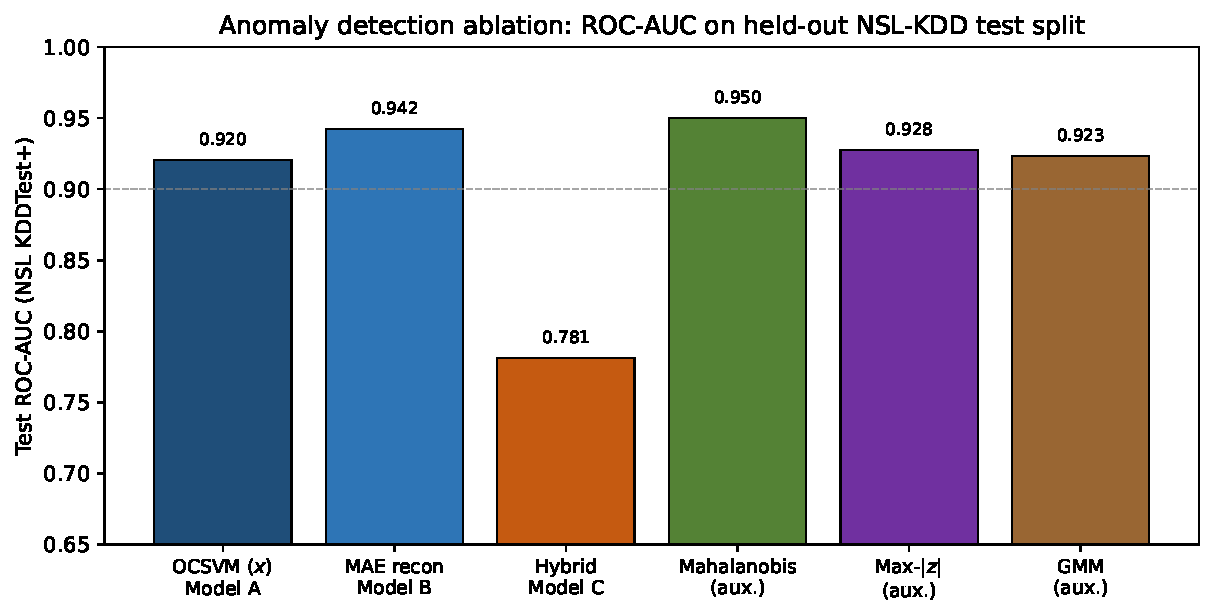
\includegraphics[width=\linewidth]{figures/generated/ablation_roc_auc.pdf}
  \caption{Test ROC-AUC comparison (values from executed notebook outputs). The hybrid underperforms single-signal models on ranking quality.}
  \label{fig:ablation}
\end{figure}

\paragraph{Reading the tables.} Model~B achieves the highest ROC-AUC among A/B/C, indicating that reconstruction error ranks normal vs.\ attack flows slightly better than the raw-feature SVM under our preprocessing. Model~A remains competitive and offers a lighter runtime profile (no neural training). Auxiliary Mahalanobis achieves the peak ROC-AUC in our suite, highlighting that elliptical distance after shrinkage is remarkably effective on this feature space---a useful sanity check for practitioners.

% ------------------------------------------------------------------
\section{Failure analysis and discussion}
\label{sec:failure}

\paragraph{Hybrid degradation (Model~C).} ROC-AUC collapses from $\approx 0.94$ to $0.78$ after convex fusion. \emph{Why?} ROC-AUC depends on the ordering of scores; min--max normalisation using only benign validation quantiles does not guarantee that reconstructed error and SVM margin are on a commensurate \emph{rank scale}. If one score preserves ordering of hard negatives better than the other, a linear mix can introduce pairwise inversions---destroying AUC while still allowing a high-precision operating point (precision $0.93$ but recall $0.72$). Formally, let $s^{(1)}_i, s^{(2)}_i$ be monotone transforms of latent margins; unless there exists a single $w$ such that $w s^{(1)} + (1-w)s^{(2)}$ is everywhere rank-consistent with the better score, AUC need not improve.

\paragraph{Mitigations.} (i)~Learn $w$ or a small MLP on validation with AUC as a surrogate; (ii)~replace linear fusion with \emph{max} or \emph{logical AND} at calibrated quantiles; (iii)~use only latent SVM if reconstruction is redundant; (iv)~copula or rank-based normalisation on the full validation distribution including attacks (careful with leakage).

\paragraph{Masked autoencoder training.} Early stopping selected weights near epoch~6 in our run---either sufficient capacity for the task or premature plateau; reporting learning curves and multiple seeds would strengthen claims.

\paragraph{Deployment path.} Offline NSL rows abstract PCAP processing; live systems would aggregate packets (e.g., via Scapy) into the same statistical schema before scoring.

% ------------------------------------------------------------------
\section{Conclusion}
\label{sec:conclusion}

We presented a semi-supervised anomaly detection stack for zero-day-style threats, combining skew-aware feature engineering, masked autoencoder reconstruction, and kernelised one-class machines on NSL-KDD. Strong ROC-AUC ($\geq 0.92$) for Models~A and~B supports the thesis that benign-only training can flag unseen attacks in flow feature space. The hybrid's AUC drop documents that \emph{integration is non-trivial}: principled fusion remains open work. Future directions include full-train NSL experiments, hyperparameter grids for $\nu$ and $\gamma$, sequence encoders over raw bytes, and drift-aware monitoring under non-stationarity \citep{mahoney2002learning}.

\paragraph{Reproducibility.} Code and notebook: repository \texttt{dl-aml-cybersec-project}; run \texttt{notebooks/phase1\_eval\_nsl\_mae\_ocsvm.ipynb} (or \texttt{jupyter nbconvert --execute} on it) and compile this report per \texttt{report/README.md}.

% ------------------------------------------------------------------
\section*{Acknowledgements}
This report was prepared as coursework at Rishihood University. We thank the open NSL-KDD mirroring community for hosting reproducible copies of the dataset.

\bibliographystyle{plainnat}
\bibliography{references}

\end{document}
